\documentclass[acmlarge,11pt,nonacm]{acmart}
\usepackage{minted}
\usepackage{tikz}
\usetikzlibrary{automata, positioning, arrows}
\tikzset{->,  % makes the edges directed
>=stealth, % makes the arrow heads bold
node distance=3cm, % specifies the minimum distance between two nodes. Change if necessary.
every state/.style={thick, fill=gray!10}, % sets the properties for each ’state’ node
initial text=$ $, % sets the text that appears on the start arrow
}
\usepackage{algorithm}
\usepackage[noend]{algpseudocode}

% Remove DOI info
\makeatletter
\renewcommand\@formatdoi[1]{\ignorespaces}
\makeatother

\settopmatter{printacmref=false} % Removes citation information below abstract
\renewcommand\footnotetextcopyrightpermission[1]{} % removes footnote with conference information in first column
\pagestyle{empty} % removes running headers

\AtBeginDocument{%
  \providecommand\BibTeX{{%
    \normalfont B\kern-0.5em{\scshape i\kern-0.25em b}\kern-0.8em\TeX}}}

\setcopyright{none}

\fancyfoot{}

\begin{document}
\title{DRILLS: Debugging RTL Intelligently with Localization from Long-Simulation}
\author{Vighnesh Iyer}
\email{vighnesh.iyer@berkeley.edu}
\author{Donggyu Kim}
\email{dgkim@berkeley.edu}
\affiliation{
  \institution{UC Berkeley}
}
\renewcommand{\shortauthors}{Iyer and Kim}

\begin{abstract}
  With increasing RTL design complexity it is increasingly difficult to debug why a subset of tests may fail in chip-level emulation.
  We propose the use of specification mining to extract a designer's assumptions about an RTL design and encode them as assertions that are checked during a failing test execution.
  Our initial results show that this technique is promising for localizing bugs in \textit{space and time} by demonstrating that the mined fine-grained LTL properties are violated before a high-level test failure condition occurs, such as timeout or hanging.
\end{abstract}
\maketitle
\thispagestyle{empty}
\section{Introduction}
Specification mining is a technique to extract LTL properties from a set of traces of signals.
This technique can be applied for several purposes in the domain of digital hardware verification including:
\begin{enumerate}
  \item Developing a suite of assertions to be used for design regressions: once a design is mature, most of the interface boundary specifications are well defined and fine-grained assertions derived from specification mining can help catch regressions when design refinements or optimizations are being made.
  \item A starting point for formally specifying a design: once a design can pass random-stimulus based and directed unit tests, specification mining can be used to extract properties that have been consistently observed in the test waveforms. These properties can then be used as assertions to prove formally.
  \item Early anomaly detection and localization on long-running tests on mature RTL: if a specific test fails on an RTL design while many other tests pass, specification mining can reveal \textit{where and when} a failing test begins to produce unusual behavior in the RTL, guiding the designer to the bug location.
\end{enumerate}
In this report, we will focus on applying specification mining to address the last point above.

\subsection{Motivation}
RTL designs are increasing in complexity and are thus more prone to having subtle bugs that are not caught in regular verification flows. Typical techniques such as randomized-stimulus testing, directed testing, and fuzz testing have a difficult time catching bugs that require the RTL be put into a very specific state.

These subtle bugs are usually caught when performing chip emulation or FPGA prototyping when running realistic workloads on the RTL.
Real workloads usually involve traces that are billion of cycles long, and are thus too slow to perform using RTL simulation which provides full design visibility.
DESSERT\cite{Kim_2018} demonstrates a technique to capture full-visibility waveform traces from fast running FPGA simulation.
Using DESSERT, an out-of-order RISC-V processor (BOOM\cite{Celio_2015}) is deterministically emulated on an FPGA with runtime assertion monitors while running the SPEC2017 benchmark suite.
During the execution of several tests, synthesized assertions were violated which revealed there exists some subtle bugs in the core causing some benchmarks to fail.

While these assertions are useful for catching errors, they are very high-level and don't direct the designer to where a bug originated.
As an example, the "\texttt{Pipeline has hung}" assertion (in BOOM) is generated with the following Chisel code:

\begin{minted}[fontsize=\small]{scala}
// detect pipeline freezes and throw error
val idle_cycles = freechips.rocketchip.util.WideCounter(32)
when (rob.io.commit.valids.asUInt.orR ||
      csr.io.csr_stall ||
      io.rocc.busy ||
      reset.asBool) {
  idle_cycles := 0.U
}
assert (!(idle_cycles.value(13)), "Pipeline has hung.")
\end{minted}

In words, this says, "If there is a good reason to stall the pipeline, reset \texttt{idle\_cycles}, otherwise let it tick up to 13 before declaring something has gone wrong."
This assertion does not give any insight as to what bad event happened, or when and where it happened.
Since these assertions are thrown after billions of cycles it is possible that some $\mu$-arch state was corrupted early in the simulation and only triggered this assertion much later during execution.
DESSERT enables extracting waveforms for a variable number of cycles before the assertion triggers, but even with the waveform dumps in hand, the designer was unable to localize the bug.
Our aim in developing this specification mining tool is to hunt out the locations of these trickly bugs in BOOM and fix them.

\subsection{Hypothesis}
Mature RTL designs (like BOOM) pass almost all tests run on them, including a full set of ISA tests, a boot of Linux, and real applications running on an OS.
If a test fails on a mature design, we hypothesize that an \textit{assumption} the designer made about the RTL was violated somewhere and at some time during the failing test execution, that was not violated on any successful test execution.
These assumptions can include believing that a certain register cannot hold certain values or higher-level properties such as: "the memory system will respond to my request within 5 cycles".

We believe specification mining can be used to extract designer assumptions about the RTL design by mining fine-grained LTL properties on waveforms of successful test executions.
These mined properties can be added to the RTL design as assertions and replaying the failing test should cause a violation of a mined property.
These violations can be used to catch a faulty assumption \textit{earlier and with greater locality} than the high-level assertions originally present in the design.

\subsection{Problem Definition}
\par
\textbf{Given}:
\begin{itemize}
  \item An RTL design driven with only one global clock
  \item A large set of VCD (value change dump) files produced when running a full suite of tests in an RTL simulator
  \item One or just a few failing tests in the suite characterized by a failed high-level assertion, hanging/global timeout, or a bad exit code
\end{itemize}
\textbf{Produce}:
\begin{itemize}
  \item A set of mined LTL properties involving signals (combinational nets and registers) of the RTL design that aren't violated on any passing test
  \item A method of ranking the mined LTL properties
  \item A program that can check a VCD against the mined properties to find any violations for that execution trace
\end{itemize}

\section{Approach}
Our plan is to first create the products above with a small RTL design.
We use \texttt{riscv-mini}\cite{riscv-mini}, a simple 3-stage in-order RISC-V processor as the RTL we will use to test the specification mining engine.
\texttt{riscv-mini} has real instruction and data caches and implements the RV32UI ISA subset which is capable of running the entire \texttt{riscv-tests}\cite{riscv-tests} test suite.
The test suite contains a comprehensive set of ISA tests and benchmarks which will be used to generate the VCD files for mining.

\subsection{Prior Work}
Specification mining has been previously applied to both software and hardware verification.
The Texada LTL spec miner\cite{Lemieux_2015} mines LTL properties from server logs and introduces the notions of confidence, support, and support potential.
Prior work\cite{Yamaguchi_2016} implemented a pre-condition miner which generated restrictions on inputs to software functions to be used for later model checking.

The main inspiration for this work comes from Wenchao Li's\cite{Li_2010}\cite{Li_2014} work on spec mining on VCD files, where four LTL templates were developed.
His work demonstrated how mined specs could detect transient and stuck-at faults in an RTL design.
We aim to extend his work for the purpose of bug localization.

There are also a host of SAT-based mux instrumentation methods\cite{Mirzaeian_2008}\cite{Smith_2005}\cite{Chang_2007} that have been explored for bug localization, primarily in space (but not time).
We believe that these techniques do not scale well with larger RTL designs and do not enable looking far back in time due to the exponential blowup of cycle unrolling.

\subsection{High-Level Flow}
The long-term plan is to leverage the spec mining engine and the prior work of DESSERT to provide an FPGA-acclererated debugging platform.
We plan to take waveforms of successful test executions from RTL simulation and FPGA emulation of BOOM and feed the spec mining engine to infer LTL properties.
The buggy RTL is instrumented by taking the LTL properties and converting them to property monitor FSMs which are stiched into the original design.
The assertions are synthesized for FPGA emulation using the same methodology described in DESSERT, and the failing tests are executed.
It is our hope that the failing tests will trigger failures in the mined properties before the failure becomes visible to the user (via a high-level assertion violation, hanging/timout, or a bad exit code).
\begin{figure}[H]
  \centering
  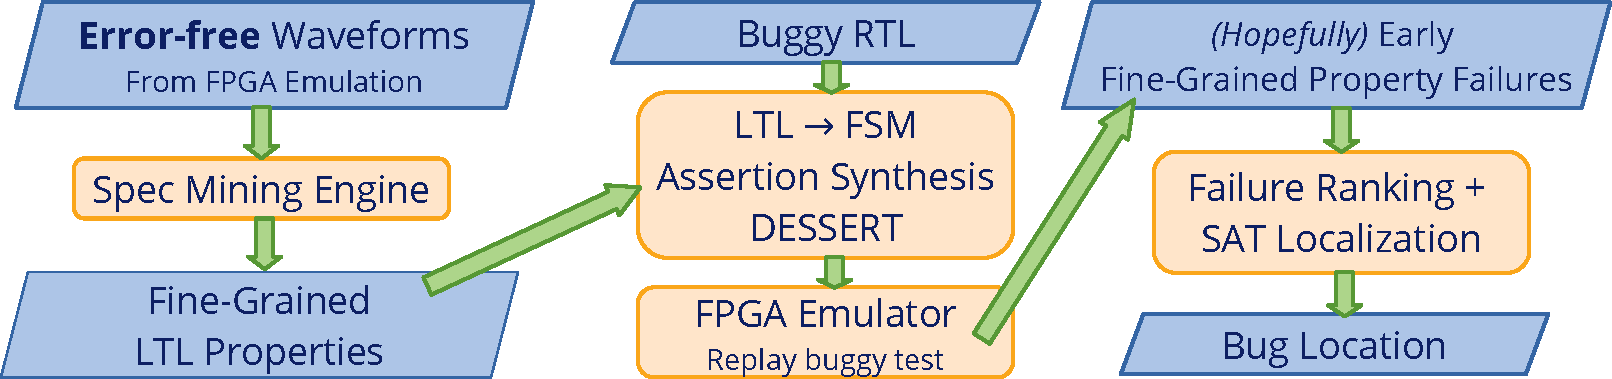
\includegraphics[width=0.8\textwidth]{figs/proposed_approach.pdf}
  \caption{The proposed tool flow to use specification mining and FPGA-accelerated simulation to pinpoint bug locations in for an RTL design .}
  \label{fig:proposed_approach}
\end{figure}
The mined properties which were violated can be ranked based on the time of their violation and we can use the SAT localization techniques mentioned above to further pinpoint the bug location.

\section{Model and Algorithms}
In this section, we will specify the formal model for LTL specification mining, how we adapted LTL formulas for RTL, and the algorithms used in the spec mining engine.

\subsection{Hardware Idioms in LTL}
They can be used to describe many common idioms present in RTL. A few examples:
\begin{itemize}
  \item There should eventually be a response (\texttt{resp}) after a request (\texttt{req}) \\
    $\quad \mathbf{G}\, (\mathtt{req} \rightarrow \mathbf{XF}\, \mathtt{resp})$
  \item There should be a response in 2 cycles after a request \\
    $\quad \mathbf{G}\, (\mathtt{req} \rightarrow \mathbf{XX}\, \mathtt{resp})$
  \item The ready/valid interface should keep \texttt{valid} high once it has been asserted until \texttt{ready} goes high \\
    $\quad \mathbf{G}\, (\mathtt{valid} \rightarrow \mathbf{X}\, (\mathtt{valid}\, \mathbf{U}\, \mathtt{ready}))$
  \item After a ready/valid transaction, the slave should be \texttt{ready} again within 2 cycles \\
    $\quad \mathbf{G}\, ((\mathtt{valid} \land \mathtt{ready}) \rightarrow (\mathbf{X}\, \mathtt{ready} \lor \mathbf{XX}\, \mathtt{ready}))$
\end{itemize}

\subsubsection{LTL Templates} \label{templates}
The formulas above can be templated by replacing the concrete signals (such as \texttt{ready}, \texttt{resp}, etc.) with variable placeholders. We consider 4 LTL templates for spec mining derived from Li's prior work\cite{Li_2014}:

\begin{itemize}
  \item Alternating: $a\, \mathbf{A}\, b$
  \item Until: $\mathbf{G}\, (a \rightarrow \mathbf{X}\, (a\, \mathbf{U}\, b))$
  \item Next: $\mathbf{G}\, (a \rightarrow \mathbf{X}\, b)$
  \item Eventual: $\mathbf{G}\, (a \rightarrow \mathbf{X F}\, b)$
\end{itemize}

where $a$ and $b$ are some boolean expressions derived from the signals in the RTL.

\subsection{Adapting LTL Templates for RTL}
RTL simulations produce a set of finite-length traces of bitvectors.
We assume that these traces are sampled on the rising edge of a given clock signal; from now on we assume all traces contain the values of signals at discrete clock cycles.
In contrast, LTL properties are defined over infinite-length traces of atomic propositions.
We convert bitvector traces to traces of \textit{delta events} which are treated as atomic propositions, and we employ notions of \textit{falsifiability} and \textit{support} to mine LTL properties on finite length traces.

Let a signal trace $\tau_i$ be a tuple of length $T$ which contains the value of the signal $i$ (a bitvector) at every discrete timestep of an RTL simulation.
Let there be $N$ signals in the RTL design: $i \in [0,N)$.
We can convert $\tau_i$ to its delta trace $\tau_{\Delta i}$ as such:
\begin{align*}
  \tau_{\Delta i}(t) = (\tau_i(t-1) \neq \tau_i(t)) \quad \forall t \in [1,T)
\end{align*}

Note that $\tau_{\Delta i}$ is a tuple of length $T-1$ and is a trace of atomic propositions.
Simply put, we convert a bitvector signal trace to a boolean trace which is 1 whenever the signal changes value, and 0 otherwise.
We now consider the templates in section \ref{templates} in the context where $a, b = \tau_{\Delta i}, \tau_{\Delta j}, i \neq j$, for some $i, j$.

Here is a concrete example where $k, q$ are bitvector signals in an RTL design where $k$ is 1 bit wide and $q$ is 10 bits wide:
\begin{align*}
  \tau_{k} &= (0, 1, 1, 1, 0) \\
  \tau_{q} &= (0, 0, 200, 200, 300) \\
  \tau_{\Delta k} &= (1, 0, 0, 1) \\
  \tau_{\Delta q} &= (0, 1, 0, 1)
\end{align*}

Note that even though $k$ is a boolean signal and can already be treated as an atomic proposition, we only mine LTL properties on its \textit{delta trace} and not the signal itself.

In RTL designs, it is usually the case that the density of transitions for a given signal is fairly low.
Signal traces can be stored in a compressed format where we only record the timestep in which the signal value changes.
Indeed, this is conveniently how traces are stored in a VCD (value change dump) file which is the input to the spec miner.
We can extract sparsely represented delta traces from a VCD file as a tuple of timesteps where the signal transitions. %of tuples where the inner tuple consists of (timestep, value) pairs.
\begin{align*}
  \tau_{\Delta k, compressed} &= (0, 3) \\
  \tau_{\Delta q, compressed} &= (1, 3)
\end{align*}

We want to consider the templates in section \ref{templates}, so we can zip 2 compressed delta traces together that indicates which of the signals transitioned.
\begin{align*}
  \tau_{\Delta k, \Delta q} &= ((\Delta k, \lnot \Delta q), (\lnot \Delta k, \Delta q), (\Delta k, \Delta q))
\end{align*}
This means that initially, $k$ transitioned and $q$ did not on a given timestep, then on a future timestep $q$ transitioned and $k$ did not, and on another future timestep both $k$ and $q$ transitioned.
Note that in this data structure, it is impossible to have a tuple where both $k$ and $q$ \textit{did not} transition.
This data structure is perfect to construct automatons that mine LTL properties.


\subsection{Mining with Automata}
We construct FSMs for each of the LTL property templates that take zipped compressed delta traces as an input.

\subsubsection{Falsifiability and Support}
A given LTL property template is \textit{falsifiable} over a zipped delta trace if its mining automaton reaches a state from which it can move to the \textit{falsified} state in one step.
We loosely define the \textit{support} for an LTL property over a trace as the number of times the pattern "repeats".
It will be made explicit in the FSMs for each LTL template as to when a pattern "repetition" occurs; we have yet to formalize this notion.
We will abbreviate falsifiable as $f$ and support as $s$.

\subsubsection{Alternating}
\begin{figure}
  \centering
  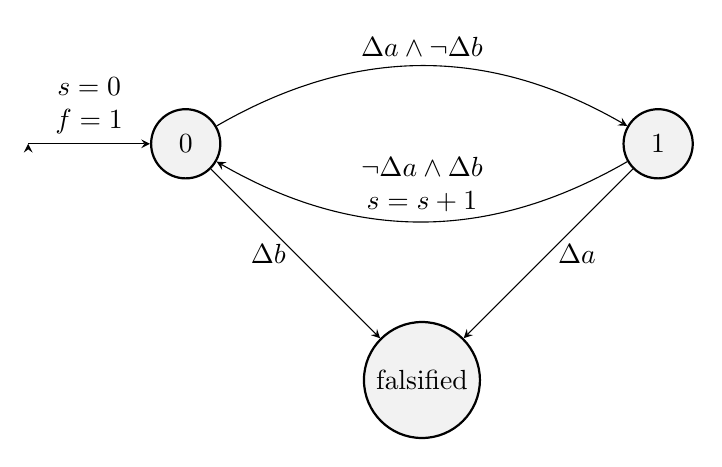
\begin{tikzpicture}
    \node[state] (q1) at (0,0) {0};
    \node[state] (q2) at (6,0) {1};
    \node[state] (q3) at (3,-3) {falsified};
    \draw (-2,0) edge[above,->] node[align=center]{$s = 0$\\$f = 1$} (q1)
    (q1) edge[bend left, above] node{$\Delta a \land \lnot \Delta b$} (q2)
    (q2) edge[bend left, above] node[align=center]{$\lnot \Delta a \land \Delta b$\\$s = s + 1$} (q1)
    (q1) edge[left] node{$\Delta b$} (q3)
    (q2) edge[right] node{$\Delta a$} (q3);
  \end{tikzpicture}
\caption{Automaton that mines the alternating LTL pattern}
\label{fig:alternating}
\end{figure}

The automaton in figure \ref{fig:alternating} mines the alternating pattern and advances support when a $\Delta a$ then $\Delta b$ sequence occurs.
This pattern is violated if $\Delta a$ and $\Delta b$ are both true on the same timestep.

\subsubsection{Until}
\begin{figure}
  \centering
  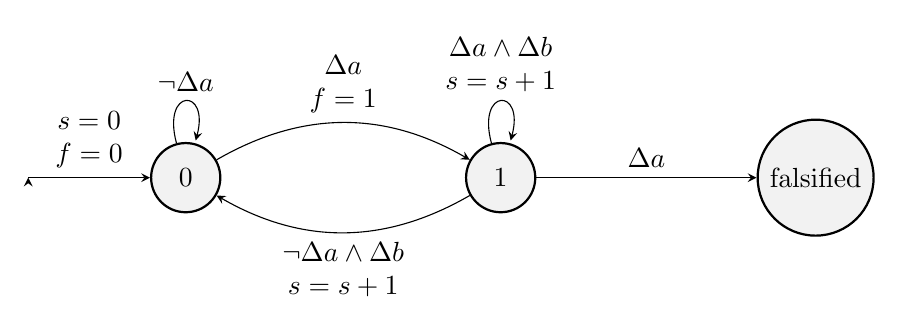
\begin{tikzpicture}
    \node[state] (q1) at (0,0) {0};
    \node[state] (q2) at (4,0) {1};
    \node[state] (q3) at (8,0) {falsified};
    \draw (-2,0) edge[above] node[align=center]{$s = 0$\\$f = 0$} (q1)
    (q1) edge[loop above] node{$\lnot \Delta a$} (q1)
    (q1) edge[bend left, above] node[align=center]{$\Delta a$\\$f = 1$} (q2)
    (q2) edge[bend left, below] node[align=center]{$\lnot \Delta a \land \Delta b$\\$s = s + 1$} (q1)
    (q2) edge[loop above] node[align=center]{$\Delta a \land \Delta b$\\$s = s + 1$} (q2)
    (q2) edge[above] node{$\Delta a$} (q3);
  \end{tikzpicture}
\caption{Automaton that mines the until LTL pattern}
\label{fig:until}
\end{figure}

The automaton in figure \ref{fig:until} mines the until pattern. If $\Delta a$ is seen 2 times in a row without a $\Delta b$ then this pattern is falsified. Note that if $\Delta a$ never occurs, this pattern can't be falsifiable on that particular delta trace.

\subsubsection{Next}
\begin{figure}
  \centering
  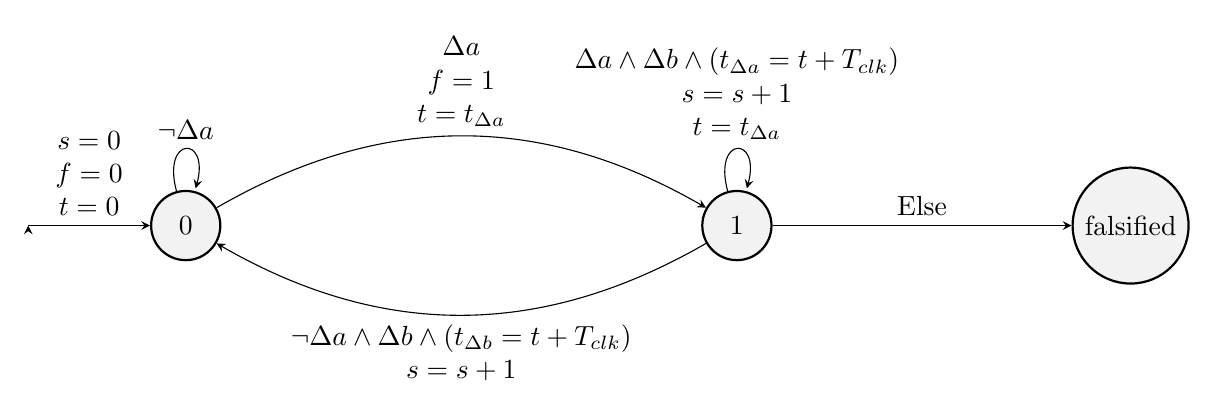
\begin{tikzpicture}
    \node[state] (q1) at (0,0) {0};
    \node[state] (q2) at (7,0) {1};
    \node[state] (q3) at (12,0) {falsified};
    \draw (-2,0) edge[above] node[align=center]{$s = 0$\\$f = 0$\\$t = 0$} (q1)
    (q1) edge[loop above] node{$\lnot \Delta a$} (q1)
    (q1) edge[bend left, above] node[align=center]{$\Delta a$\\$f = 1$\\$t = t_{\Delta a}$} (q2)
    (q2) edge[bend left, below] node[align=center]{$\lnot \Delta a \land \Delta b \land (t_{\Delta b} = t + T_{clk})$\\$s = s + 1$} (q1)
    (q2) edge[loop above] node[align=center]{$\Delta a \land \Delta b \land (t_{\Delta a} = t + T_{clk})$\\$s = s + 1$\\$t = t_{\Delta a}$} (q2)
    (q2) edge[above] node{Else} (q3);
  \end{tikzpicture}
\caption{Automaton that mines the next LTL pattern}
\label{fig:next}
\end{figure}

Some hacking is needed with the next automaton in figure \ref{fig:next} to constrain the pattern to only be valid when $\Delta b$ happens after 1 clock cycle after $\Delta a$.
The variables $t_{\Delta a}$ and $t_{\Delta b}$ represent the time at which the $a$ and $b$ delta events occured on the transitions in which they are used.
Let $T_{clk}$ be the clock period, and $t$ is a state variable to hold the transition time of $a$.

\subsubsection{Eventual}
\begin{figure}
  \centering
  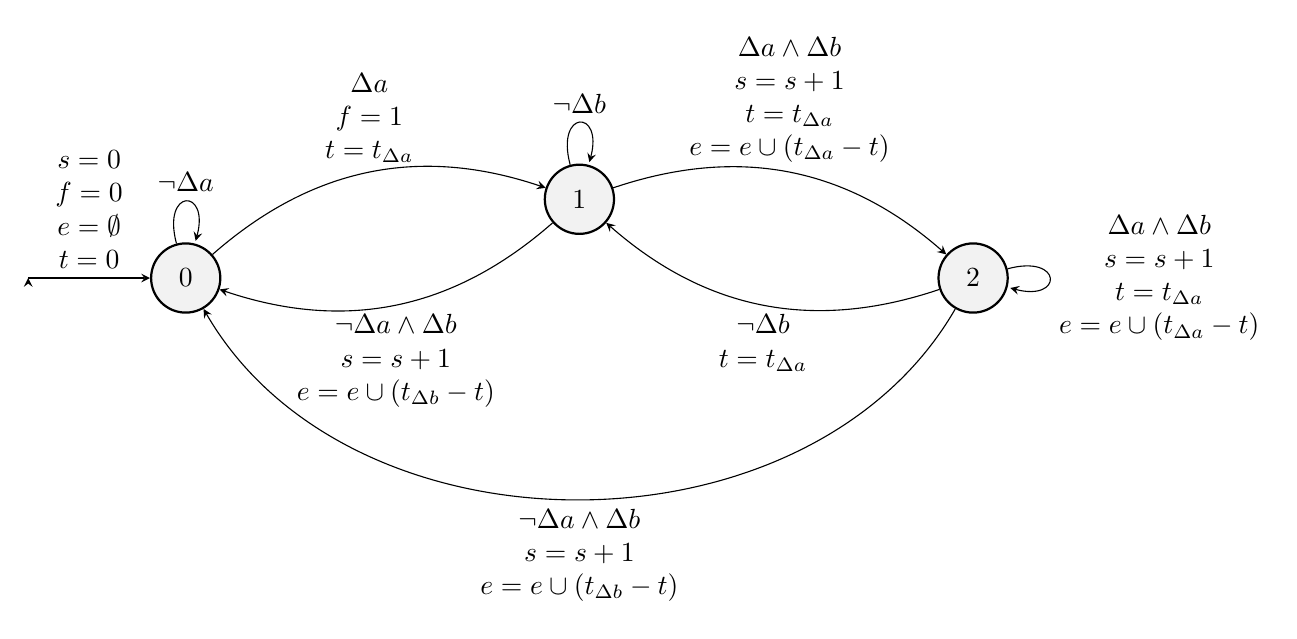
\begin{tikzpicture}
    \node[state] (q0) at (0,0) {0};
    \node[state] (q2) at (10,0) {2};
    \node[state] (q1) at (5,1) {1};
    \draw
    (-2,0) edge[above] node[align=center]{$s = 0$\\$f = 0$\\$e = \emptyset$\\$t = 0$} (q0)
    (q0) edge[loop above] node{$\lnot \Delta a$} (q0)
    (q0) edge[bend left, above] node[align=center]{$\Delta a$\\$f = 1$\\$t = t_{\Delta a}$} (q1)
    (q1) edge[bend left, below] node[align=center]{$\lnot \Delta a \land \Delta b$\\$s = s + 1$\\$e = e \cup (t_{\Delta b} - t)$} (q0)
    (q1) edge[loop above] node{$\lnot \Delta b$} (q1)
    (q1) edge[bend left, above] node[align=center]{$\Delta a \land \Delta b$\\$s = s + 1$\\$t = t_{\Delta a}$\\$e = e \cup (t_{\Delta a} - t)$} (q2)
    (q2) edge[loop right] node[align=center]{$\Delta a \land \Delta b$\\$s = s + 1$\\$t = t_{\Delta a}$\\$e = e \cup (t_{\Delta a} - t)$} (q2)
    (q2) edge[bend left, below] node[align=center]{$\lnot \Delta b$\\$t = t_{\Delta a}$} (q1)
    (q2) edge[bend left=60, below] node[align=center]{$\lnot \Delta a \land \Delta b$\\$s = s + 1$\\$e = e \cup (t_{\Delta b} - t)$} (q0)
    ;
  \end{tikzpicture}
\caption{Automaton that mines the eventual LTL pattern}
\label{fig:eventual}
\end{figure}

Note that the eventual pattern is never falsifiable on a finite-length trace as seen in figure \ref{fig:eventual}.
In addition to simply keeping track of the \textit{support} we also maintain a set of times it took to get to $\Delta b$ from $\Delta a$.
This allows us to empirically find cycle limits for the eventual pattern so it can reasonably be applied to finite-length traces.

\subsection{Naive Mining Algorithm}
The algorithm we used to mine LTL properties on VCD files is very naive, but is still relatively fast due to the sparsity of the compressed delta traces and the limited set of signals that can fill the roles of $a$ and $b$ in the LTL templates.
\begin{algorithm}[H]
  \caption{Naive Spec Miner}
  \begin{algorithmic}[1]
    \Procedure{Miner}{$[\tau_{\Delta 1,c}, \dots, \tau_{\Delta N,c}], M$} \Comment{$M$ is the RTL module hierarchy}
      \State $P \gets \emptyset$
      \For{$[\tau_m] \leftarrow$ \Call{Modularize}{$[\tau_{\Delta 1,\dots,N,c}]$, M}} \Comment{Split traces by module}
        \State $[\tau_{m,trim}] \gets$ \Call{Trim}{$[\tau_m]$} \Comment{Only keep signals with width $\leq$ 5 bits}
        \If{$\lnot$ \Call{IsLeaf}{m}} \Comment{Only consider port signals except for leaf modules}
          \State $[\tau_{m,trim}] \gets$ \Call{StripInternal}{$[\tau_{m,trim}]$}
        \EndIf
        \For{$(\tau_{\Delta i}, \tau_{\Delta j}) \leftarrow$ \Call{Permutations}{$[\tau_{m,trim}], 2$}}
          \For{$\text{Miner} \leftarrow [\mathbf{A, N, U, E}]$}
            \State $P \gets P \; \cup$ \Call{Miner}{$\tau_{\Delta i}, \tau_{\Delta j}$}
          \EndFor
        \EndFor
      \EndFor
      \State \textbf{return} $P$
    \EndProcedure
  \end{algorithmic}
\end{algorithm}

The algorithm begins by splitting delta traces along module boundaries via DFS and furthermore constrains the signals under consideration to be below 5 bits in width and in the module's port list (except for leaf modules).
Usually this technique keeps the final length of $\tau_{m,trim}$ to below 10 which makes iterating over their permutations ($\mathcal{O}(n!)$) have reasonable runtime.
We maintain a set of mined properties that is updated as the miner proceeds along different modules.

\subsection{Merging Properties and Checking}
For each VCD we add a property to the mined set $P$ if the miner reports it as \textit{falsifiable} and is either \textit{falsified} or has positive \textit{support}.
Properties mined from each VCD are the merged together into a final property set by discarding any properties that were \textit{falsified} at any time and aggregating the \textit{support} for any properties that were never falsified.

The final property set can be fed into a checker which will run the the miner for each property on a VCD trace and verify that none of them are falsified.

\subsection{Challenges}
Most of the challenges for this project were engineering-related.
We had to hand construct automaton for each of the LTL templates and check them against many test inputs to verify they accurately captured the property.
The automaton had to work with compressed delta trace inputs which complicates some of the checks for the next and until patterns.

\section{Results}
We apply our specification mining engine to \texttt{riscv-mini} which has the module hierarchy and number of signals in table \ref{tab:riscv-mini}.
\begin{table}
  \caption{Module hierarchy, number of signals under consideration for mining for \texttt{riscv-mini}, and mined properties for 2 ISA tests}
  \label{tab:riscv-mini}
  \begin{tabular}{llll}
    \toprule
    Module & Number of Signals & Props Mined on add & Props Mined on sw\\
    \midrule
    TOP & 4 & 45 & 45 \\
    TOP.Tile & 15 & 791 & 1529 \\
    TOP.Tile.icache & 18 & 1113 & 1113 \\
    TOP.Tile.dcache & 4 & 43 & 1965 \\
    TOP.Tile.core & 12 & 565 & 973 \\
    TOP.Tile.core.dpath & 23 & 2149 & 3308 \\
    TOP.Tile.core.dpath.regFile & 4 & 43 & 43\\
    TOP.Tile.core.dpath.immGen & 1 & 0 & 0 \\
    TOP.Tile.core.dpath.csr & 16 & 849 & 1080 \\
    TOP.Tile.core.dpath.brCond & 8 & 261 & 261\\
    TOP.Tile.core.dpath.alu & 3 & 24 & 24 \\
    TOP.Tile.core.ctrl & 9 & 333 & 403 \\
    TOP.Tile.arb & 11 & 430 & 683 \\
  \bottomrule
  \end{tabular}
\end{table}
% How many specs were mined, how did the spec merging evolve the mined specs as more VCDs were added?
% How many of each spec type were mined?
% How many specs resided in each module?

We also record the number of properties mined for each module for 2 different tests that stress different parts of the processor.
The \texttt{add} test does not stress the memory system and data cache as much as the \texttt{sw} test and this can be seen in the modules where the discrepency between the number of mined properties is highest.

We mined properties on all VCD traces produced by the \texttt{riscv-mini} ISA test suite and merged them together.
When merging properties, many of them are falsified and we are left with only \textbf{3251} properties at the end.
Here is an exerpt of the mined properties with the highest support:

\begin{minted}[breaklines, fontsize=\footnotesize]{text}
Until TOP.Tile.core.ctrl.io_A_sel -> TOP.Tile.core.dpath.io_ctrl_imm_sel, support: 6113
Next TOP.Tile.core.dpath.brCond.eq -> TOP.Tile.core.dpath.brCond.neq, support: 5457
Eventual TOP.Tile.core.dpath.io_ctrl_imm_sel -> TOP.Tile.core.dpath.regFile_io_wen, support: 4466
Until TOP.Tile.icache.io_cpu_req_valid -> TOP.Tile.icache.is_idle, support: 4359
Until TOP.Tile.icache.io_cpu_req_valid -> TOP.Tile.icache.is_read, support: 4359
Eventual TOP.Tile.icache.io_cpu_req_valid -> TOP.Tile.icache.is_read, support: 4336
Until TOP.Tile.icache.io_cpu_req_valid -> TOP.Tile.core.dpath.csr_io_stall, support: 4318
\end{minted}

Some of these properties are interesting, but ultimately many of them are redundant or obvious (such as mining next on a shift register).
Some of the properties that a human designer would identify as valuable have lower levels of support, such as:

\begin{minted}[breaklines, fontsize=\footnotesize]{text}
Next TOP.Tile.core.dpath.csr.isEcall -> TOP.Tile.dcache_io_cpu_abort, support: 45
\end{minted}

The reader may notice that these properties appear to be mined across module boundaries, contrary to the algorithm as stated.
This is because many signals are aliased across module boundaries and the mined properties printout just shows one alias of the signal.

\subsection{Bug Localization}
We introduce a bug in \texttt{Control.scala} that mimics a copy/paste bug:
\begin{minted}{scala}
   io.csr_cmd := ctrlSignals(11)
-  io.illegal := ctrlSignals(12)
+  io.illegal := ctrlSignals(11)
\end{minted}
This bug caused the \texttt{sub} ISA test to hang, so after letting it time out, the failing VCD was checked against the mined properties.
\begin{minted}[breaklines, fontsize=\footnotesize]{text}
ERROR on property Until TOP.Tile.core.dpath.csr.io_illegal -> TOP.Tile.icache.io_cpu_req_valid
ERROR on property Until TOP.Tile.core.dpath.csr.io_illegal -> TOP.Tile.icache.io_cpu_resp_valid
ERROR on property Until TOP.Tile.core.dpath.csr.io_illegal -> TOP.Tile.core.ctrl.io_A_sel
\end{minted}

The violated properties directly point to something wrong with the \texttt{io\_illegal} signal, and effectively localize the bug.

We introduced another bug in \texttt{Cache.scala}:
\begin{minted}{scala}
-  hit := v(idx_reg) && rmeta.tag === tag_reg
+  hit := v(idx_reg) && rmeta.tag =/= tag_reg
\end{minted}

This bug does not affect most ISA tests but a multiply benchmark failed via hanging.
After checking the VCD against the mined properties, we found these violations ranked by time of violation:
\begin{minted}[breaklines, fontsize=\scriptsize]{text}
ERROR on property Until TOP.Tile.arb_io_dcache_r_ready -> TOP.Tile.dcache.hit with support 24 at time 418
ERROR on property Until TOP.Tile.dcache_io_nasti_r_valid -> TOP.Tile.dcache.hit with support 24 at time 418
ERROR on property Until TOP.Tile.dcache.is_alloc -> TOP.Tile.dcache.hit with support 24 at time 418
ERROR on property Until TOP.Tile.arb.io_dcache_ar_ready -> TOP.Tile.arb_io_nasti_r_ready with support 4173 at time 640
\end{minted}

Yet again, the violated properties point to something wrong with the \texttt{hit} signal and localize the bug.

\subsection{Future Work}
There are quite a few things to improve:
\begin{itemize}
  \item Add additional LTL templates that mine on boolean signal traces and delta event traces
  \item Prune away mined properties that are statically provable (such as shift registers)
  \item Develop a faster VCD parser to allow mining over larger VCD files
  \item Generalize the miner to take any LTL formula and automatically construct an automaton to mine the template
  \item Construct traces of atomic propositions from user-defined events (such as ready/valid transactions firing)
  \item Introduce more subtle bugs in \texttt{riscv-mini} and check whether they can be caught
\end{itemize}

\section{Course-Related Stuff}
Donggyu provided the inspiration and motivation for this project and gave suggestions on what types of bugs to introduce in \texttt{riscv-mini}.
Vighnesh implemented the spec mining engine and evaluated it on \texttt{riscv-mini}.

This project makes use of LTL specifications and conversion of an LTL formula to an automaton.
We thank Prof. Seshia for introducing a wide variety of topics in this course and for his advice on our project.

Our project is \href{https://github.com/vighneshiyer/spec-mining/}{available on Github}.

\bibliographystyle{ACM-Reference-Format}
\bibliography{references}

\end{document}
\endinput
